\documentclass[aspectratio=169,10pt]{beamer}
\usepackage[brazil]{babel}
\usepackage{beamerthemeResearchUNIFESP}
\usepackage{graphicx,booktabs,array,tikz}
\usetikzlibrary{arrows.meta,positioning,fit,calc}
\graphicspath{{figures/}}

\title[TCC Apresentação]{Predição de propriedades para materiais\\2D usando aprendizado contrastivo}
\subtitle{\small Apresentação de Trabalho de Conclusão de Curso (TCC)}
\author[Luis Filipe Menezes]{%
  \small Luis Filipe Menezes \and Marcos G. Quiles}
\institute[UNIFESP]{%
  \small
  Instituto de Ciência e Tecnologia, Universidade Federal de São Paulo -- UNIFESP}
\date{Apresentação --Novembro de 2026}

\newcommand{\smallsource}[1]{{\vspace{1mm}\tiny\color{ResearchGray}#1}}
\newcommand{\metric}[3]{%
  \begin{beamercolorbox}[rounded=true,sep=1.1ex,wd=\linewidth]{block body}
    {\scriptsize\color{ResearchGray}#1}\par
    {\Large\bfseries\color{ResearchGreenDark}#2}\par
    {\scriptsize #3}
  \end{beamercolorbox}}
\newcommand{\tightitem}{\setlength{\itemsep}{3pt}\setlength{\parskip}{0pt}}

\begin{document}

\begin{frame}[plain]
  \titlepage
\end{frame}

\begin{frame}{Contextualização}
\begin{columns}[T,onlytextwidth]
  \column{.45\textwidth}
  \begin{itemize}\tightitem
    \item Materiais 2D apresentam espessura atômica e confinamento quântico.
    \item São candidatos para eletrônica, fotovoltaica, catálise e armazenamento de energia.
    \item Propriedades físico-químicas relevantes incluem estabilidade, \emph{band gap} ($E_g$) e energia de formação.
  \end{itemize}
  \vspace{1.5mm}
  \begin{block}{Desafio}
    Explorar milhares de combinações químicas e estruturais exige métodos rápidos e escaláveis.
  \end{block}
  \column{.5\textwidth}
  \begin{figure}
    \centering
    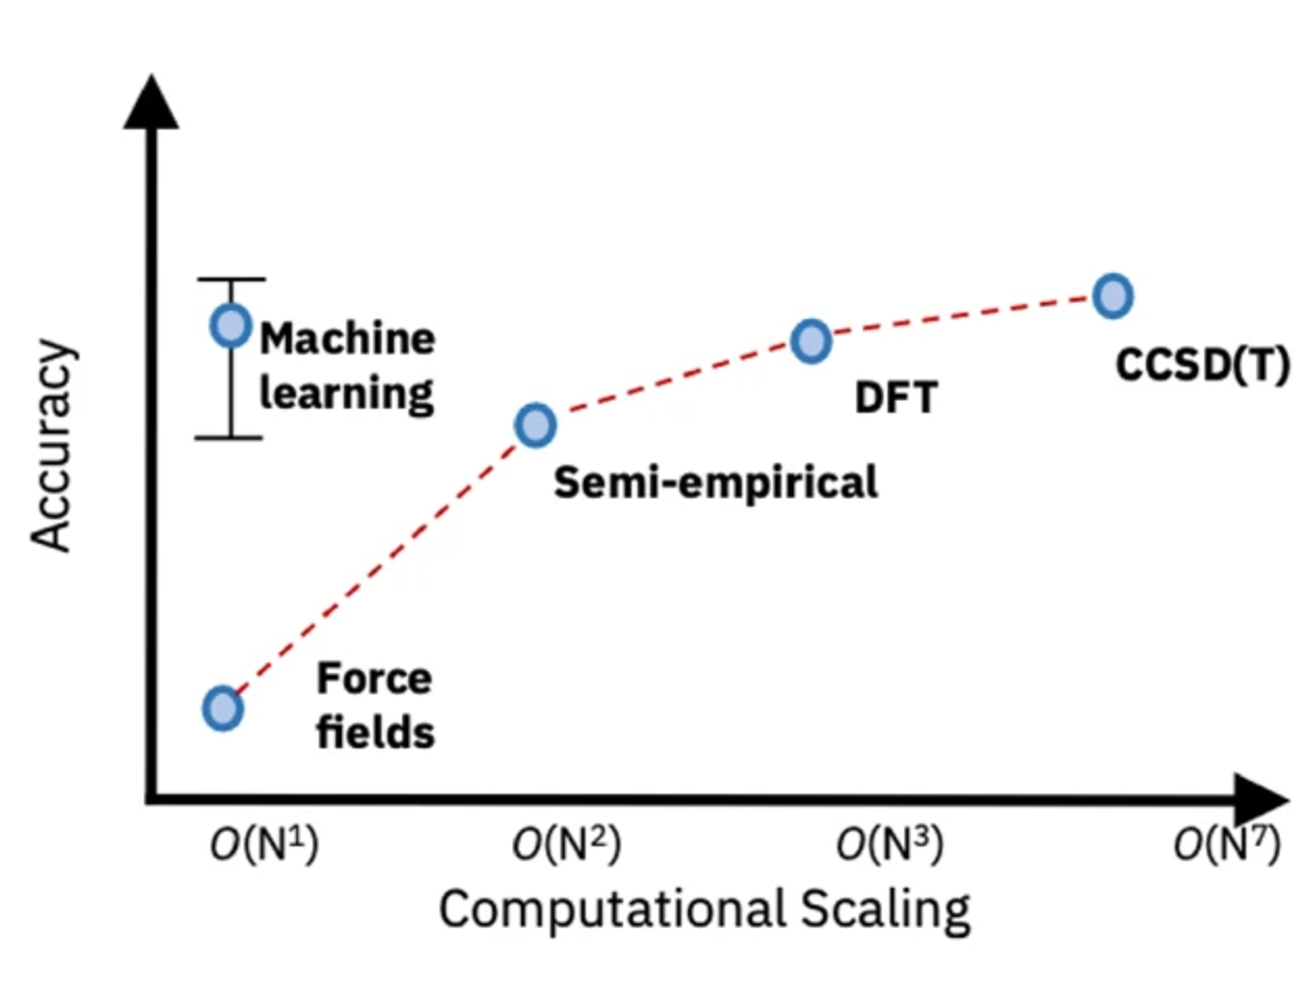
\includegraphics[width=.9\linewidth]{figures/computational_scale.pdf}
    \caption{\scriptsize Custo computacional e acurácia atrelada ao cálculo de propriedades físicas\cite{PyzerKnapp2022}.}
  \end{figure}
  % \begin{beamercolorbox}[rounded=true,sep=1.2ex,wd=\linewidth]{block body}
  %   \centering
  %   \textbf{C2DB}\\[1mm]
  %   {\small base especializada em monocamadas 2D caracterizadas por DFT}
  % \end{beamercolorbox}
\end{columns}
% \smallsource{Fontes: introdução e revisão bibliográfica da monografia.}
\end{frame}

\begin{frame}{Problema de pesquisa}
\begin{columns}[T,onlytextwidth]
  \column{.48\textwidth}
  \begin{block}{Custo computacional de DFT}
  \begin{itemize}\tightitem
    \item Resolve iterativamente as equações de Kohn--Sham.
    \item Escala com o número de átomos e a complexidade da célula $O(N^3)$.
    % \item VASP, PBE e HSE06 têm custos muito diferentes.
  \end{itemize}
  \end{block}
  \column{.48\textwidth}
  \begin{block}{Limitação dos dados supervisionados}
  \begin{itemize}\tightitem
    \item Rótulos de alta fidelidade são escassos.
    \item Redes profundas podem apresentar \textit{overfitting}.
    \item A generalização fora da distribuição é difícil (\textit{exploitation}).
  \end{itemize}
  \end{block}
\end{columns}
\vspace{4mm}
\centering
\textbf{Pergunta central:} como aprender representações estruturais úteis com poucos rótulos?
\end{frame}

  % \begin{frame}{Objetivos}
  % \begin{block}{Objetivo geral}
  % Desenvolver, implementar e avaliar modelos contrastivos para predizer propriedades físico-químicas de materiais 2D.
  % \end{block}
  % \vspace{2mm}
  % \begin{columns}[T,onlytextwidth]
  %   \column{.49\textwidth}
  %   \begin{itemize}\tightitem
  %     \item Revisar aprendizado contrastivo auto-supervisionado e supervisionado.
  %     \item Pré-processar estruturas da C2DB em representações adequadas.
  %   \end{itemize}
  %   \column{.49\textwidth}
  %   \begin{itemize}\tightitem
  %     \item Implementar redes siamesas e codificadores baseados em similaridade.
  %     \item Avaliar representações latentes em tarefas downstream.
  %   \end{itemize}
  % \end{columns}
  % \vspace{3mm}
  % \centering
  % \textbf{Propriedades-alvo:} $E_g$ (\emph{band gap}) e $\Delta H$ (energia de formação).
  % \end{frame}

\begin{frame}{Aprendizado contrastivo}
\begin{columns}[T,onlytextwidth]
  \column{.43\textwidth}
  \begin{figure}
    \centering
    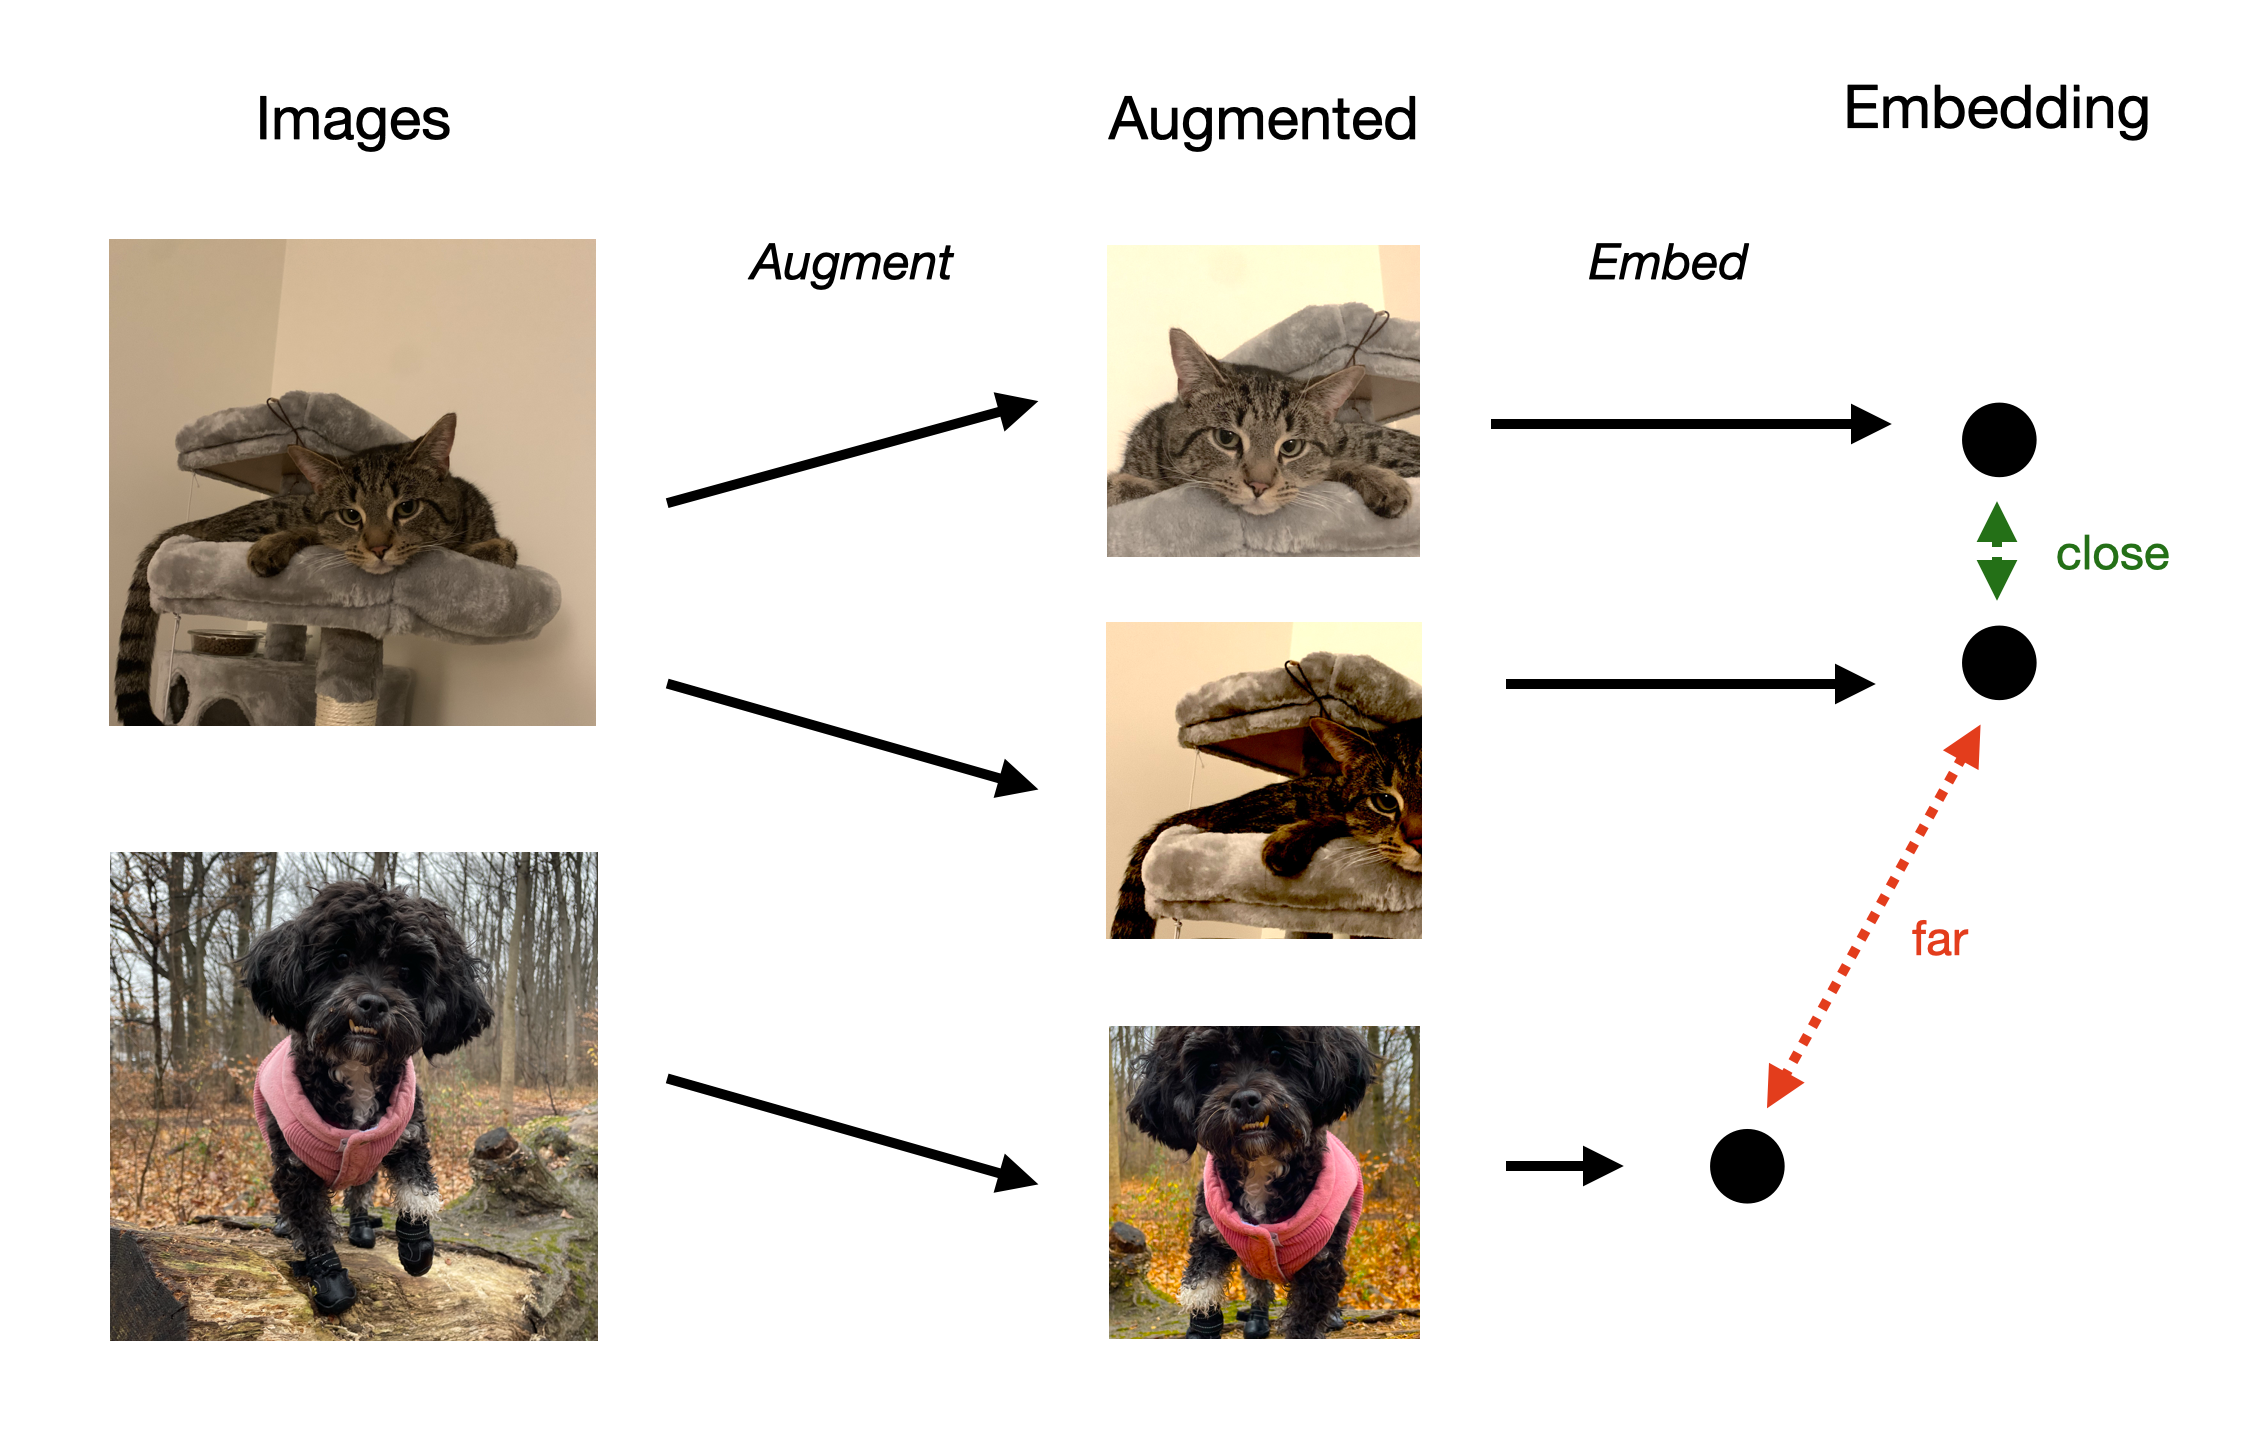
\includegraphics[width=.9\linewidth]{figures/contrastive_standard.png}
    \caption{\scriptsize Aproximação de pares positivos e afastamento de negativos.}
  \end{figure}
  \column{.53\textwidth}
  \begin{block}{Ideia central}
  Projetar amostras semelhantes próximas e amostras distintas afastadas em um espaço latente.
  \end{block}
  \[
  d_{\cos}(z_i,z_j)=1-
  \frac{z_i^\top z_j}{\|z_i\|_2\|z_j\|_2}
  \]
  \begin{itemize}\tightitem
    \item \textbf{Positivos:} vistas da mesma estrutura ou exemplos da mesma faixa de propriedade.
    \item \textbf{Negativos:} outras estruturas ou propriedades distintas.
  \end{itemize}
\end{columns}
\end{frame}

\begin{frame}{Abordagens contrastivas}
\begin{columns}[T,onlytextwidth]
  \column{.48\textwidth}
  \begin{block}{Auto-supervisionada}
  \begin{itemize}\tightitem
    \item Não usa rótulos físicos.
    \item SimCLR/NT-Xent usa vistas aumentadas da mesma amostra.
    \item CLIP (Contrastive Language-Image Pretraining) usa pares multimodais (texto e imagem).
    % \item Aprende invariâncias estruturais.
  \end{itemize}
  \end{block}
  \column{.48\textwidth}
  \begin{figure}
    \centering
    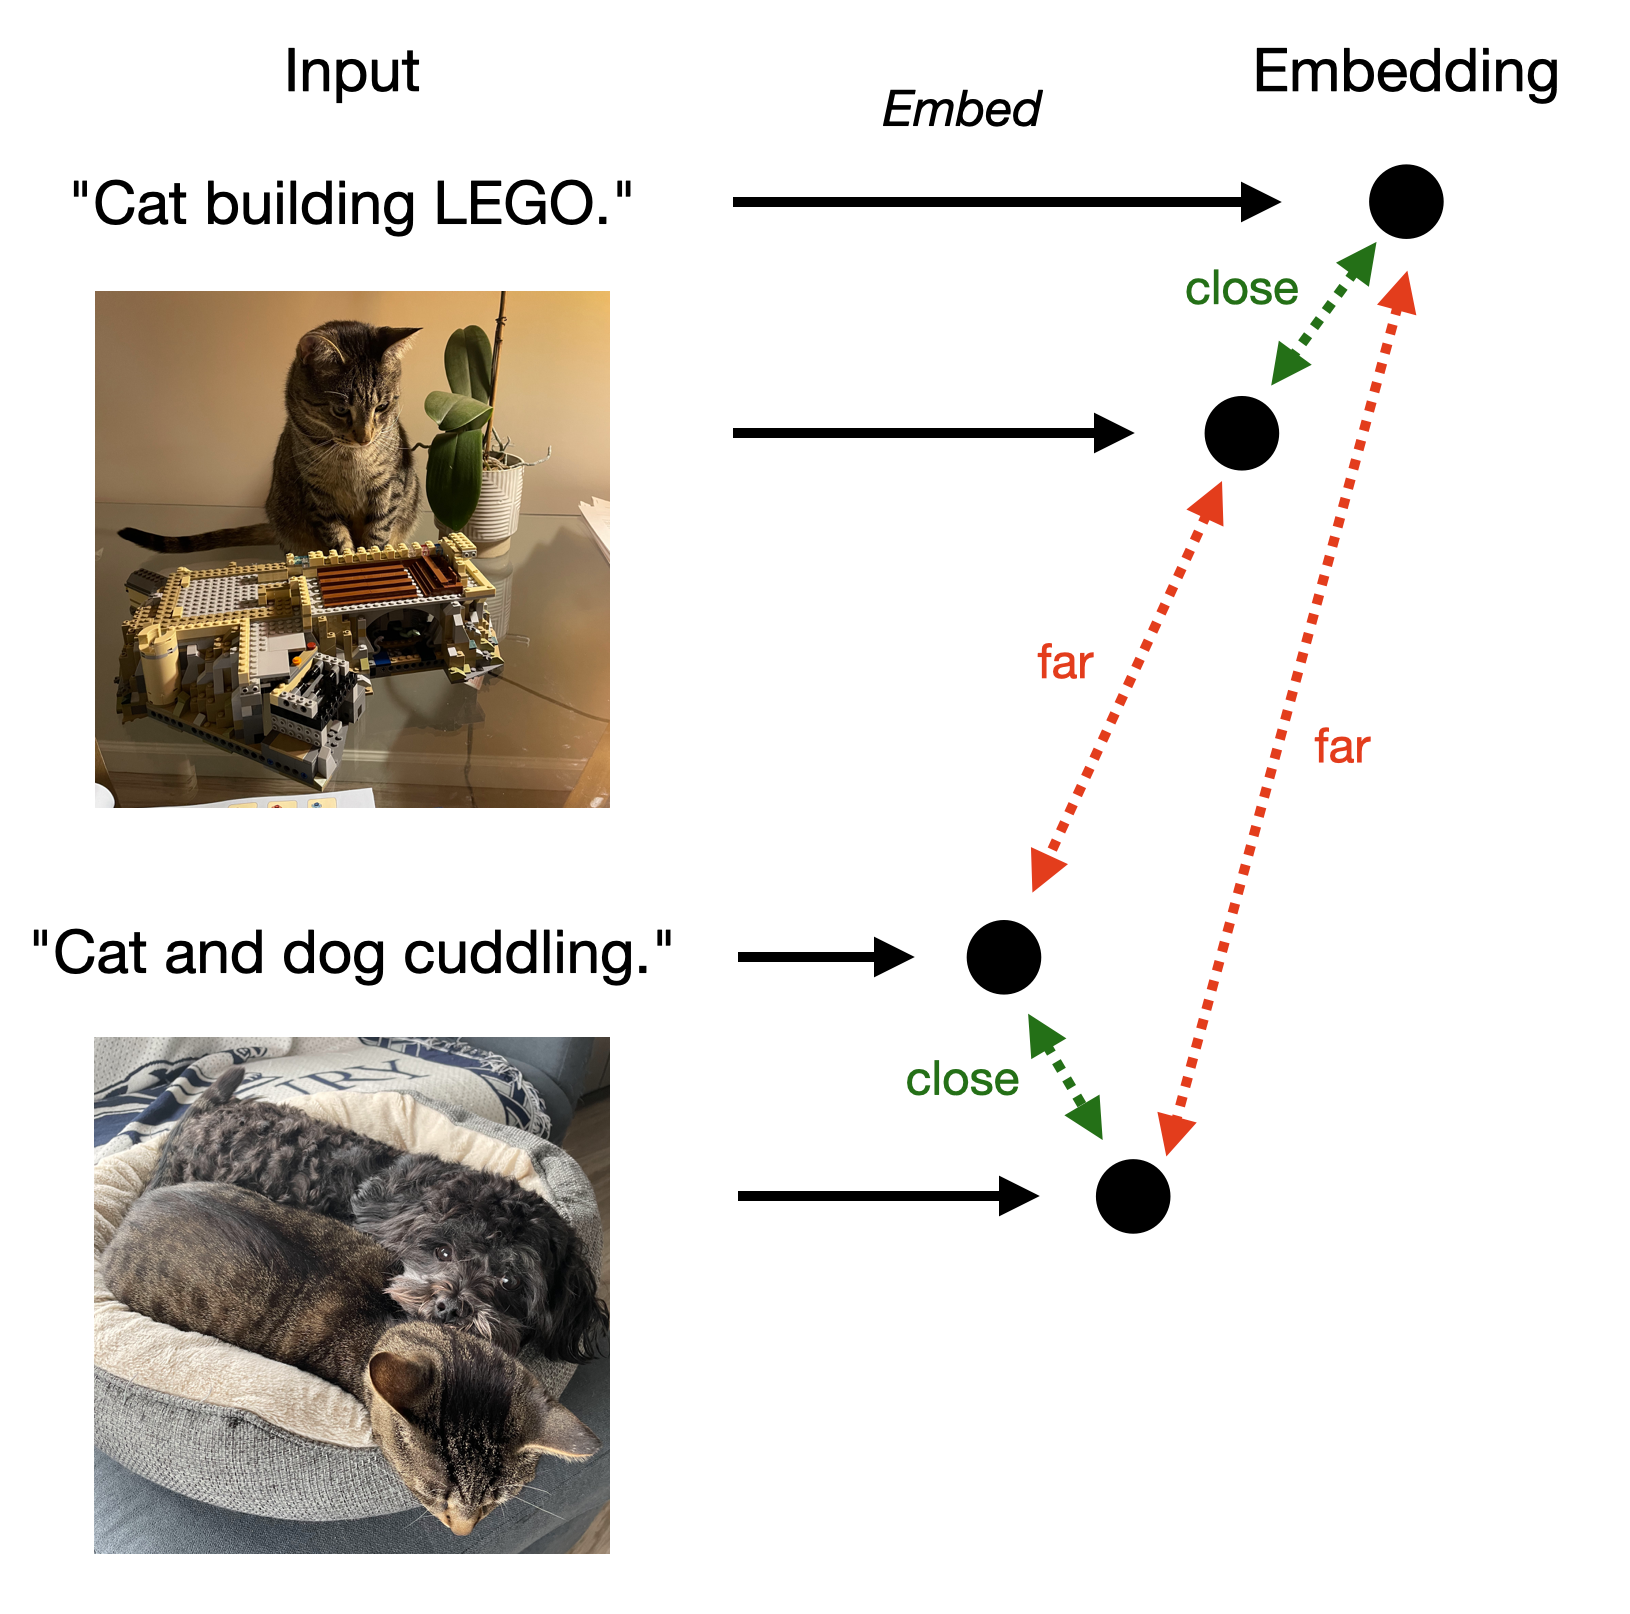
\includegraphics[width=.75\linewidth]{figures/contrastive_CLIP.png}
    \caption{\scriptsize CLIP utilizando pares multimodais para determinar similaridade entre textos e imagens.}
  \end{figure}
\end{columns}
\end{frame}

\begin{frame}{Abordagens contrastivas}
\begin{columns}[T,onlytextwidth]
  \column{.48\textwidth}
  \begin{block}{Supervisionada SupCon}
  \begin{itemize}\tightitem
    \item Usa rótulos ou faixas de propriedades.
    \item Cada amostra pode ter múltiplos positivos.
    \item Organiza o espaço conforme semelhanças funcionales.
  \end{itemize}
  \end{block}
  \column{.4\textwidth}
  \begin{tikzpicture}[
    node distance=2mm,
    box/.style={rounded corners,draw=ResearchGreen,fill=white,minimum height=8mm,align=center,font=\scriptsize},
    sample/.style={rounded corners,minimum width=17mm,minimum height=9mm,align=center,font=\tiny},
    flow/.style={-{Stealth[length=1.5mm]},draw=ResearchGray,line width=.6pt}
  ]
  \node[box,minimum width=43mm] (data) {Lote de grafos rotulados $(G_k,y_k)$};
  \node[box,below=of data,minimum width=40mm] (encoder) {GNN compartilhada\\+ projetor};
  \node[sample,below=5mm of encoder,draw=ResearchGreen,fill=ResearchGreen!10] (positive) {Positivo\\$z_p,\ y_p=0$};
  \node[sample,left=5.0mm of positive,draw=ResearchGreenDark,fill=ResearchGreen!10] (anchor) {Âncora\\$z_i,\ y_i=0$};
  \node[sample,right=5mm of positive,draw=orange!80!black,fill=orange!10] (negative) {Negativo\\$z_n,\ y_n=1$};
  \draw[flow] (data) -- (encoder);
  \draw[flow] (encoder.south) -- (anchor.north);
  \draw[flow] (encoder.south) -- (positive.north);
  \draw[flow] (encoder.south) -- (negative.north);
  % \node[below=2mm of positive,align=center,font=\tiny,text=ResearchGreenDark] (relations)
    % {Mesmo rótulo: positivos \quad Rótulo distinto: negativo};
  \node[below=1mm of positive,align=center,font=\scriptsize,text=ResearchGreenDark]
    {Função de custo \textbf{aproxima} $z_i,z_p$\\e \textbf{afasta} $z_i,z_n$};
  \end{tikzpicture}
\end{columns}
\vspace{4mm}
% \centering
% \textbf{Transição proposta:} pré-treinar sem rótulos e ajustar pesos para regressão específica.
\end{frame}


\begin{frame}{Representação estrutural por grafos}
\begin{columns}[T,onlytextwidth]
  \column{.43\textwidth}
  \begin{block}{Grafo cristalino $G=(V,E)$}
  \begin{itemize}\tightitem
    \item Nós $V$: átomos e características periódicas.
    \item Arestas $E$: ligações ou distâncias interatômicas.
  \end{itemize}
  \end{block}
  \begin{block}{Codificadores considerados}
  \begin{itemize}\tightitem
    \item CGCNN\cite{Xie2017CGCNN} %: passagem de mensagens em grafos cristalinos.
    \item ALIGNN %: grafos atômicos e de linhas.
    \item Equiformer %: equivariância rotacional e representações direcionais.
  \end{itemize}
  \end{block}
  \column{.53\textwidth}
  \begin{figure}
    \centering
    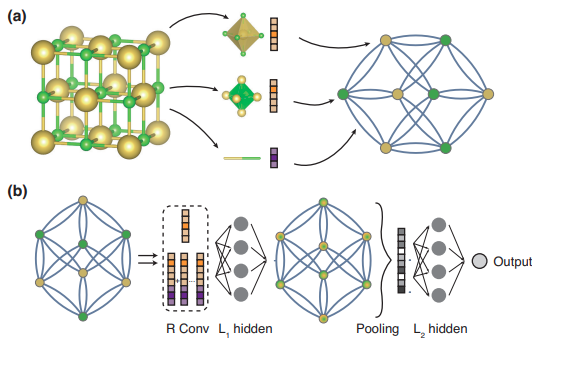
\includegraphics[width=.9\linewidth]{figures/GNN.png}
    \caption{\scriptsize Representação de uma monocamada 2D como grafo.}
  \end{figure}
  \vspace{2mm}
  % \smallsource{A estrutura deve preservar invariância translacional, rotacional e permutacional.}
\end{columns}
\end{frame}

\begin{frame}{Revisão bibliográfica sintetizada}
\begin{columns}[T,onlytextwidth]
  \column{.31\textwidth}
  \begin{beamercolorbox}[rounded=true,sep=1.2ex,wd=\linewidth]{block body}
    \centering\textbf{\color{ResearchGreenDark}Aprendizado contrastivo}\\[2mm]
    {\scriptsize SimCLR, NT-Xent, SupCon e Graph Contrastive Learning}
  \end{beamercolorbox}
  \column{.31\textwidth}
  \begin{beamercolorbox}[rounded=true,sep=1.2ex,wd=\linewidth]{block body}
    \centering\textbf{\color{ResearchGreenDark}Representações}\\[2mm]
    {\scriptsize CGCNN, ALIGNN, Equiformer e descritores como SOAP/MBTR}
  \end{beamercolorbox}
  \column{.31\textwidth}
  \begin{beamercolorbox}[rounded=true,sep=1.2ex,wd=\linewidth]{block body}
    \centering\textbf{\color{ResearchGreenDark}Ciência dos materiais}\\[2mm]
    {\scriptsize CrystalCLR, C2DB, JARVIS-2D e modelos foundation}
  \end{beamercolorbox}
\end{columns}
\vspace{5mm}
\centering
\textbf{Convergência metodológica:} GNN + transformações físicas + perda contrastiva.
\smallsource{Principais referências: Koker et al. (2022), Chen et al. (2020), Khosla et al. (2020), Xie e Grossman (2018).}
\end{frame}

\begin{frame}{Metodologia proposta -- visão geral}
\centering
\begin{tikzpicture}[node distance=5mm,
  phase/.style={rounded corners,draw=ResearchGreen,fill=white,minimum height=14mm,minimum width=30mm,align=center,font=\scriptsize},
  arrow/.style={-{Stealth[length=2mm]},line width=.7pt,ResearchGreen}]

  \node[phase] (data) {\textbf{C2DB}\\Estruturas 2D};
  \node[phase,right=of data] (pre) {\textbf{Pré-processamento}\\Grafo $G=(V,E)$};
  \node[phase,right=of pre] (aug) {\textbf{Aumentações}\\Vistas $\tilde G_i,\tilde G_j$};
  \node[phase,right=of aug] (gnn) {\textbf{Codificador GNN}\\Pesos compartilhados};
  \node[phase,right=of gnn] (lat) {\textbf{Espaço latente}\\$z_i,z_j$};
  \node[phase,right=of lat] (loss) {\textbf{Perda contrastiva}\\NT-Xent / SupCon};

  \draw[arrow] (data)--(pre);
  \draw[arrow] (pre)--(aug);
  \draw[arrow] (aug)--(gnn);
  \draw[arrow] (gnn)--(lat);
  \draw[arrow] (lat)--(loss);

  \node[below=12mm of gnn,phase,minimum width=38mm] (ft) {\textbf{Ajuste fino}\\Regressor MLP};
  \node[below=12mm of lat,phase,minimum width=38mm] (prop) {\textbf{Propriedades}\\$E_g$, $\Delta H$};
  \draw[arrow] (gnn.south) -- (ft.north);
  \draw[arrow] (ft)--(prop);
\end{tikzpicture}
\vspace{2mm}
\textbf{Dois ramos:} auto-supervisionado por vistas estruturais e supervisionado por rótulos/faixas.
\end{frame}

\begin{frame}{Pré-processamento e aumentações}
\begin{columns}[T,onlytextwidth]
  \column{.49\textwidth}
  \begin{block}{Conversão em grafos}
  \begin{itemize}\tightitem
    \item Extrair estruturas cristalinas da C2DB.
    \item Representar átomos como nós.
    \item Representar ligações e distâncias como arestas.
  \end{itemize}
  \end{block}
  \column{.49\textwidth}
  \begin{block}{Aumentações fisicamente plausíveis}
  \begin{itemize}\tightitem
    \item Pequenas perturbações atômicas.
    \item Deformações elásticas no plano da monocamada.
    \item Operações que preservem composição e coerência física.
  \end{itemize}
  \end{block}
\end{columns}
\vspace{3mm}
\centering
\textbf{Risco metodológico:} aumentações excessivas podem criar estruturas não representativas.
\end{frame}

\begin{frame}{Treinamento contrastivo}
\begin{columns}[T,onlytextwidth]
  \column{.49\textwidth}
  \begin{block}{Ramo auto-supervisionado}
  \[
  \mathcal L_{\mathrm{NT-Xent}}
  =-\log
  \frac{\exp(\mathrm{sim}(z_i,z_j)/\tau)}
  {\sum_{k\neq i}\exp(\mathrm{sim}(z_i,z_k)/\tau)}
  \]
  \begin{itemize}\tightitem
    \item Pares positivos: duas vistas da mesma estrutura.
    \item Pares negativos: demais estruturas do lote.
  \end{itemize}
  \end{block}
  \column{.49\textwidth}
  \begin{block}{Ramo supervisionado}
  \begin{itemize}\tightitem
    \item SupCon usa amostras com propriedades semelhantes.
    \item Para regressão, propriedades podem ser discretizadas em faixas.
    \item Os pesos podem ser transferidos ao regressor downstream.
  \end{itemize}
  \end{block}
\end{columns}
\end{frame}

\begin{frame}{Avaliação proposta}
\begin{columns}[T,onlytextwidth]
  \column{.54\textwidth}
  \begin{block}{Tarefas downstream}
  \begin{itemize}\tightitem
    \item Regressão do \emph{band gap} $E_g$.
    \item Regressão da energia de formação $\Delta H$.
    \item Comparação com CGCNN supervisionado diretamente.
  \end{itemize}
  \end{block}
  \vspace{2mm}
  \begin{block}{Protocolo}
  \begin{itemize}\tightitem
    \item Separação treino, validação e teste.
    \item Busca de arquitetura, temperatura e taxa de aprendizado.
  \end{itemize}
  \end{block}
  \column{.42\textwidth}
  \metric{Métrica principal}{MAE}{Erro médio absoluto em eV}
  \vspace{2mm}
  \metric{Métricas adicionais}{$R^2$, RMSE}{Generalização e magnitude do erro}
\end{columns}
\smallsource{A validação deve evitar vazamento entre composições ou estruturas semelhantes.}
\end{frame}

\begin{frame}{Resultados esperados e contribuições}
\begin{columns}[T,onlytextwidth]
  \column{.49\textwidth}
  \begin{block}{Hipótese investigada}
  O pré-treinamento contrastivo produz representações latentes mais informativas que descritores manuais e supera o treinamento puramente supervisionado em cenários com poucos rótulos.
  \end{block}
  \column{.49\textwidth}
  \begin{block}{Contribuições esperadas}
  \begin{itemize}\tightitem
    \item Adaptação de aprendizado contrastivo para materiais 2D.
    \item Pipeline reproduzível com a C2DB.
    \item Comparação entre contraste supervisionado e auto-supervisionado.
  \end{itemize}
  \end{block}
\end{columns}
\vspace{4mm}
\centering
\textbf{Limitação central:} a precisão também depende da qualidade dos rótulos DFT utilizados.
\end{frame}

\begin{frame}[plain]
  \begin{tikzpicture}[remember picture,overlay]
    \node[anchor=north east,xshift=-8mm,yshift=-7mm]
      at (current page.north east) {\cinelogo};
  \end{tikzpicture}
  \vspace{10mm}
  {\usebeamerfont{title}\color{ResearchGreenDark}Conclusão}
  \vspace{5mm}
  \begin{itemize}\tightitem
    \item O custo da DFT limita a varredura de candidatos 2D.
    \item Grafos representam átomos e interações de forma estruturalmente rica.
    \item Aprendizado contrastivo pode aprender representações úteis com poucos rótulos.
    \item A proposta combina pré-treinamento contrastivo e regressão de $E_g$ e $\Delta H$.
  \end{itemize}
  \vfill
  \centering
  {\Large\bfseries\color{ResearchGreenDark}Obrigado!}\\[2mm]
  Perguntas
\end{frame}
\begin{frame}{Referências}
  \bibliographystyle{splncs04}
  \bibliography{paper_source/biblio}
\end{frame}
\end{document}
